\section{Function Approximation}


\subsection{Problem 5.9}


\begin{figure}[!ht]
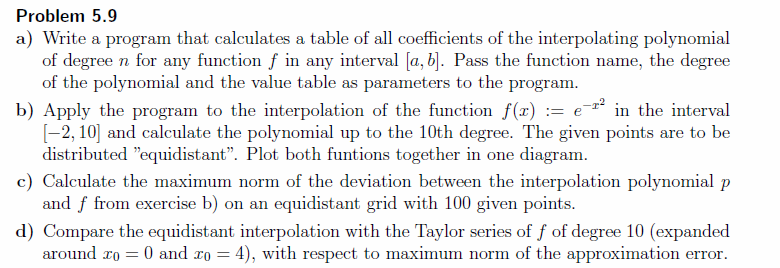
\includegraphics[width=1\textwidth]{chapters/images/desc-5-9}
\end{figure}



\subsubsection{a)}

X

\begin{lstlisting}[caption=todo]
def getCoefficients(fx, degree, a, b):
	xses = [];
	yses = [];
	
	step = (b - a) / float(degree - 1);
	
	for i in range(degree):
		x = a + i * step;
		xses.append(x);
		yses.append(fx(x));
	
	matA = [];
	
	for xVal in xses:
		row = [];
		for i in range(degree):
			row.append(pow(xVal, i));
		
		matA.append(row);
	
	matrixArr = np.array(matA);
	vectorArr = np.array(yses);
	
	linSolutions = np.linalg.solve(matrixArr, vectorArr);
	
	return linSolutions;
#
\end{lstlisting}


results:

\begin{lstlisting}[caption=Result of 1.1 a), keywordstyle=\color{black}]
R
\end{lstlisting}

X



\subsubsection{b)}

X

\begin{lstlisting}[caption=todo]

def polynomialF(coefficients, x):
	sum = 0.0;
	
	for i in range(len(coefficients)):
		sum += coefficients[i] * pow(x, i);
	
	return sum;
#

def myF(x):
	return pow(math.e, -pow(x, 2));
#


coefficients = getCoefficients(myF, 10, -2, 10);

xses = [];
realYses = [];
approxYses = [];

for i in range(100):
	x = -2 + i * (12 / 100.0);
	
	xses.append(x);
	realYses.append(myF(x));
	approxYses.append(polynomialF(coefficients, x));


plt.plot(xses, realYses);
plt.plot(xses, approxYses);
plt.xlabel("x");
plt.ylabel("y");
plt.show();
\end{lstlisting}


results:

\begin{figure}[!ht]
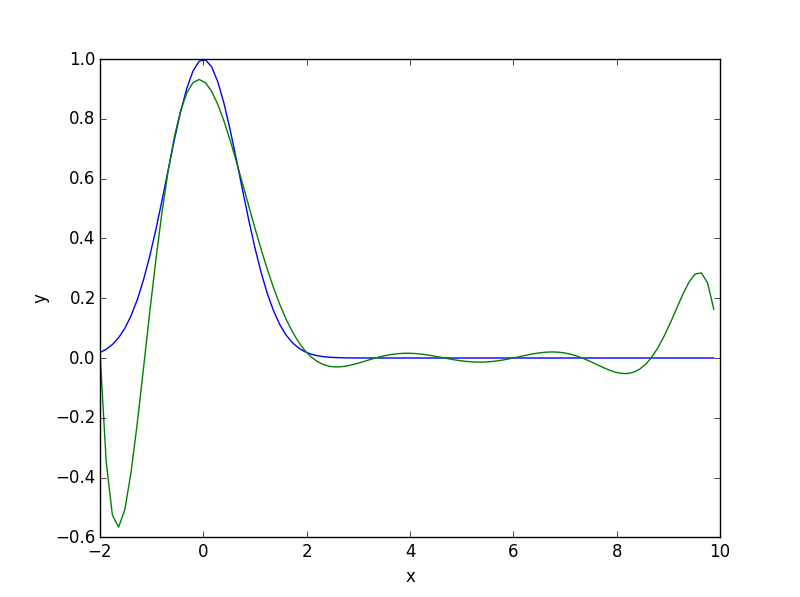
\includegraphics[width=1\textwidth]{chapters/images/figure-5-9-b}
\caption{todo}
\end{figure}


X



\subsubsection{c)}

X

\begin{lstlisting}[caption=todo]

maxApproxDev = -1;

for i in range(100):
	realY = realYses[i];
	approxY = approxYses[i];
	
	maxApproxDev = max(maxApproxDev, abs(realY - approxY));


print("maximum deviation: " + str(maxApproxDev));

\end{lstlisting}


results:

\begin{lstlisting}[caption=Result of 1.1 a), keywordstyle=\color{black}]
maximum deviation: 0.634025332357
\end{lstlisting}

X



\subsubsection{d)}

X

\begin{lstlisting}[caption=todo]


def taylorFuncAt0(x):
	sum = 1;
	sum -= pow(x, 2);
	sum += pow(x, 4) / 2.0;
	sum -= pow(x, 6) / 6.0;
	sum += pow(x, 8) / 24.0;
	sum -= pow(x, 10) / 120.0;
	sum += pow(x, 12) / 720.0;
	sum -= pow(x, 14) / 5040.0;
	sum += pow(x, 16) / 40320.0;
	
	return sum;
#

def taylorFuncAt4(x):
	ep16 = float(pow(math.e, 16));
	xm4 = x - 4;
	
	sum = 1 / ep16;
	sum -= 8 * xm4 / ep16;
	sum += 31 * pow(xm4, 2) / ep16;
	sum -= 232 * pow(xm4, 3) / (3 * ep16);
	sum += 835 * pow(xm4, 4) / (6 * ep16);
	sum -= 2876 * pow(xm4, 5) / (15 * ep16);
	sum += 18833 * pow(xm4, 6) / (90 * ep16);
	sum -= 58076 * pow(xm4, 7) / (315 * ep16);
	sum += 332777 * pow(xm4, 8) / (2520 * ep16);
	sum -= 43325 * pow(xm4, 9) / (567 * ep16);
	sum += 3937007 * pow(xm4, 10) / (113400 * ep16);
	
	return sum;
#

taylor0Yses = [];
taylor4Yses = [];

for i in range(100):
	x = -2 + i * (12 / 100.0);
	
	taylor0Yses.append(taylorFuncAt0(x));
	taylor4Yses.append(taylorFuncAt4(x));


maxTaylor0Dev = -1;
maxTaylor4Dev = -1;

for i in range(100):
	realY = realYses[i];
	taylor0Y = taylor0Yses[i];
	taylor4Y = taylor4Yses[i];
	
	maxTaylor0Dev = max(maxTaylor0Dev, abs(realY - taylor0Y));
	maxTaylor4Dev = max(maxTaylor4Dev, abs(realY - taylor4Y));


print("maximum deviation of taylor series with c = 0: " + str(maxTaylor0Dev));
print("maximum deviation of taylor series with c = 4: " + str(maxTaylor4Dev));
\end{lstlisting}


results:

\begin{lstlisting}[caption=Result of 1.1 a), keywordstyle=\color{black}]
maximum deviation of taylor series with c = 0: 1.88827128486e+11
maximum deviation of taylor series with c = 4: 354.936464804
\end{lstlisting}

X








\subsection{Problem 5.10}


\begin{figure}[!ht]
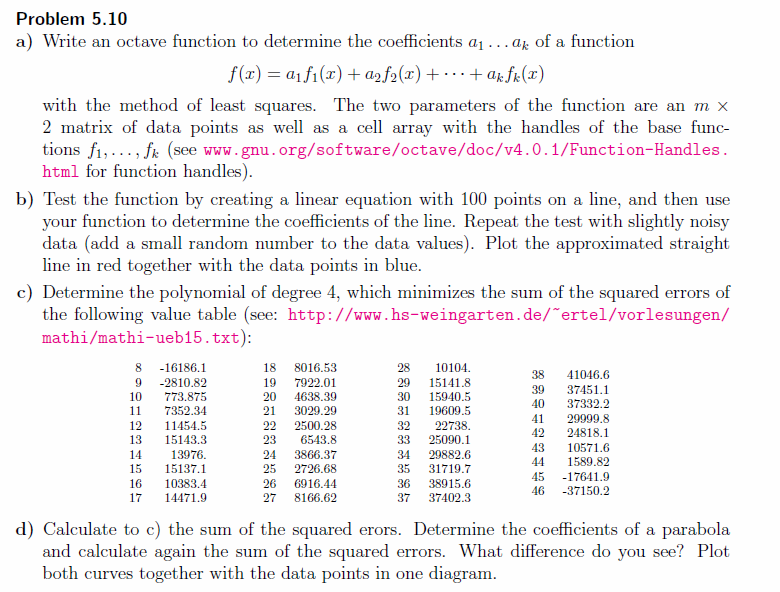
\includegraphics[width=1\textwidth]{chapters/images/desc-5-10}
\end{figure}




\subsubsection{a)}

X

\begin{lstlisting}[caption=todo]

def getCoefficients(baseFunctions, dataPoints):
	l = len(baseFunctions);
	
	matA = [];
	
	for i in range(l):
		matrixRow = [];
		for j in range(l):
			elemSum = 0;
		
			for dp in dataPoints:
				x = dp[0];
				elemSum += baseFunctions[i](x) * baseFunctions[j](x);
			
			matrixRow.append(elemSum);
		
		matA.append(matrixRow);
	
	vecB = [];
	
	for i in range(l):
		elemSum = 0;
	
		for dp in dataPoints:
			elemSum += dp[1] * baseFunctions[i](dp[0]);
		
		vecB.append(elemSum);
	
	
	matrixArr = np.array(matA);
	vectorArr = np.array(vecB);
	
	linSolutions = np.linalg.solve(matrixArr, vectorArr);
	
	return linSolutions;
#

\end{lstlisting}



X


\subsubsection{b)}

X

\begin{lstlisting}[caption=todo]
def myF2(x): return pow(x, 2);

def myF1(x): return x;

def myF0(x): return 1;

baseFns = [];

baseFns.append(myF1);
baseFns.append(myF0);

linPoints = [];
rndPoints = [];
xses = [];
yses = [];
rndYses = [];

for i in range(100):
	x = i / 10.0;
	y = x * 0.64 + 2.3;
	
	xses.append(x);
	yses.append(y);

	rnd = random.random() - 0.5;
	rndY = y + rnd * 0.6;
	rndYses.append(rndY);
	
	linPoints.append([x, y]);
	rndPoints.append([x, rndY]);


print("coefficients:");
print(getCoefficients(baseFns, linPoints));

print("approximated coefficients:");
print(getCoefficients(baseFns, rndPoints));


plt.plot(xses, yses);
plt.plot(xses, rndYses, "ro");
plt.xlabel("x");
plt.ylabel("y");
plt.show();

\end{lstlisting}


results:

\begin{lstlisting}[caption=Result of 1.1 a), keywordstyle=\color{black}]
coefficients:
[ 0.64   0.23 ]

approximated coefficients:
[ 0.63139257   2.33442881 ]
\end{lstlisting}

X

\begin{figure}[!ht]
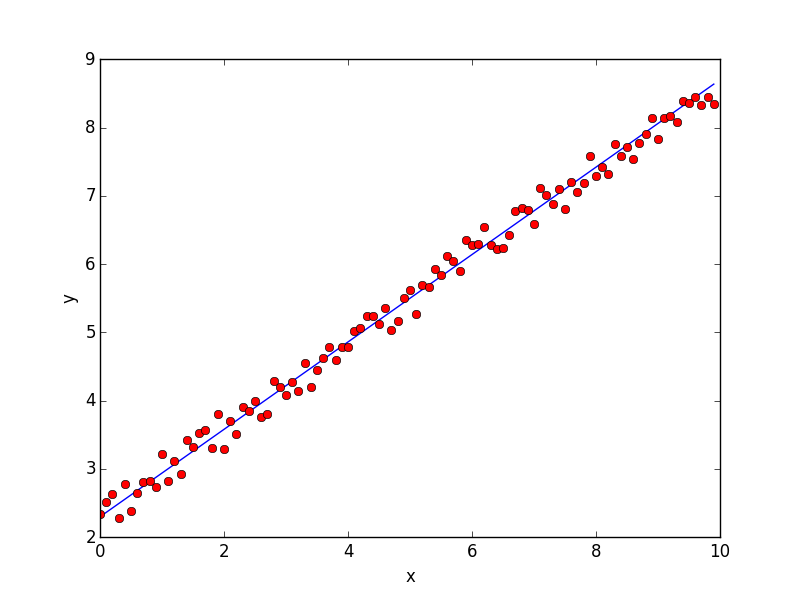
\includegraphics[width=1\textwidth]{chapters/images/figure-5-10-b}
\caption{todo}
\end{figure}






\subsubsection{c)}

X

\begin{lstlisting}[caption=todo]


def myF4(x): return pow(x, 4);
def myF3(x): return pow(x, 3);
def myF2(x): return pow(x, 2);
def myF1(x): return x;
def myF0(x): return 1;


def polynomialF(coefficients, x):
	sum = 0.0;
	
	nc = len(coefficients);
	
	for i in range(nc):
		sum += coefficients[i] * pow(x, nc - i - 1);
	
	return sum;
#

txtBaseFns4 = [];
txtBaseFns2 = [];

txtBaseFns4.append(myF4);
txtBaseFns4.append(myF3);
txtBaseFns4.append(myF2);
txtBaseFns4.append(myF1);
txtBaseFns4.append(myF0);

txtBaseFns2.append(myF2);
txtBaseFns2.append(myF1);
txtBaseFns2.append(myF0);

txtPoints = [];

txtPoints.append([8, -16186.1]);
txtPoints.append([9, -2810.82]);
txtPoints.append([10, 773.875]);
txtPoints.append([11, 7352.34]);
txtPoints.append([12, 11454.5]);
txtPoints.append([13, 15143.3]);
txtPoints.append([14, 13976.]);
txtPoints.append([15, 15137.1]);
txtPoints.append([16, 10383.4]);
txtPoints.append([17, 14471.9]);
txtPoints.append([18, 8016.53]);
txtPoints.append([19, 7922.01]);
txtPoints.append([20, 4638.39]);
txtPoints.append([21, 3029.29]);
txtPoints.append([22, 2500.28]);
txtPoints.append([23, 6543.8]);
txtPoints.append([24, 3866.37]);
txtPoints.append([25, 2726.68]);
txtPoints.append([26, 6916.44]);
txtPoints.append([27, 8166.62]);
txtPoints.append([28, 10104.]);
txtPoints.append([29, 15141.8]);
txtPoints.append([30, 15940.5]);
txtPoints.append([31, 19609.5]);
txtPoints.append([32, 22738.]);
txtPoints.append([33, 25090.1]);
txtPoints.append([34, 29882.6]);
txtPoints.append([35, 31719.7]);
txtPoints.append([36, 38915.6]);
txtPoints.append([37, 37402.3]);
txtPoints.append([38, 41046.6]);
txtPoints.append([39, 37451.1]);
txtPoints.append([40, 37332.2]);
txtPoints.append([41, 29999.8]);
txtPoints.append([42, 24818.1]);
txtPoints.append([43, 10571.6]);
txtPoints.append([44, 1589.82]);
txtPoints.append([45, -17641.9]);
txtPoints.append([46, -37150.2]);

txtCoefficients4 = getCoefficients(txtBaseFns4, txtPoints);
txtCoefficients2 = getCoefficients(txtBaseFns2, txtPoints);

txtPointsXses = [];
txtPointsYses = [];

error4 = 0;
error2 = 0;

for i in range(len(txtPoints)):
	txtPoint = txtPoints[i];
	
	txtPointsXses.append(txtPoint[0]);
	txtPointsYses.append(txtPoint[1]);
	
	y4 = polynomialF(txtCoefficients4, i + 8);
	y2 = polynomialF(txtCoefficients2, i + 8);
	
	error4 += pow(y4 - txtPoint[1], 2);
	error2 += pow(y2 - txtPoint[1], 2);


print("error of degree 4 polynomial: " + str(error4));
print("error of degree 2 polynomial: " + str(error2));

txtFXses = [];
txtF4Yses = [];
txtF2Yses = [];

for i in range(152):
	x = 8 + i * 0.25;
	
	txtFXses.append(x);
	
	y4 = polynomialF(txtCoefficients4, x);
	y2 = polynomialF(txtCoefficients2, x);
	
	txtF4Yses.append(y4);
	txtF2Yses.append(y2);


plt.plot(txtFXses, txtF4Yses);
plt.plot(txtFXses, txtF2Yses);
plt.plot(txtPointsXses, txtPointsYses, "ro");
plt.xlabel("x");
plt.ylabel("y");
plt.show();

\end{lstlisting}


results:

\begin{lstlisting}[caption=Result of 1.1 a), keywordstyle=\color{black}]
R
\end{lstlisting}

X



\subsubsection{d)}

siehe c) - aufdröseln

\begin{lstlisting}[caption=todo]

C

\end{lstlisting}


results:

\begin{lstlisting}[caption=Result of 1.1 a), keywordstyle=\color{black}]
error of degree 4 polynomial: 101457690.277
error of degree 2 polynomial: 7711489909.2
\end{lstlisting}

X


\begin{figure}[!ht]
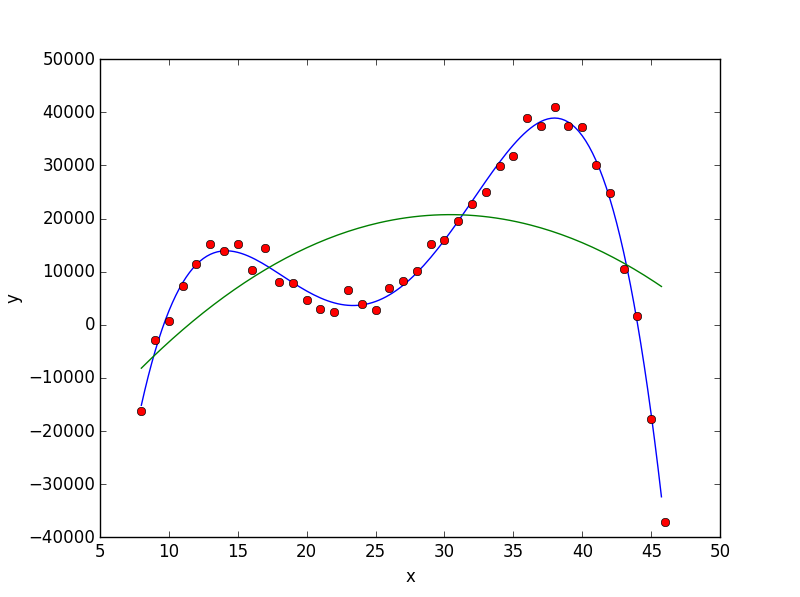
\includegraphics[width=1\textwidth]{chapters/images/figure-5-10-d}
\caption{todo}
\end{figure}

Y









\subsection{Problem 5.11}


\begin{figure}[!ht]
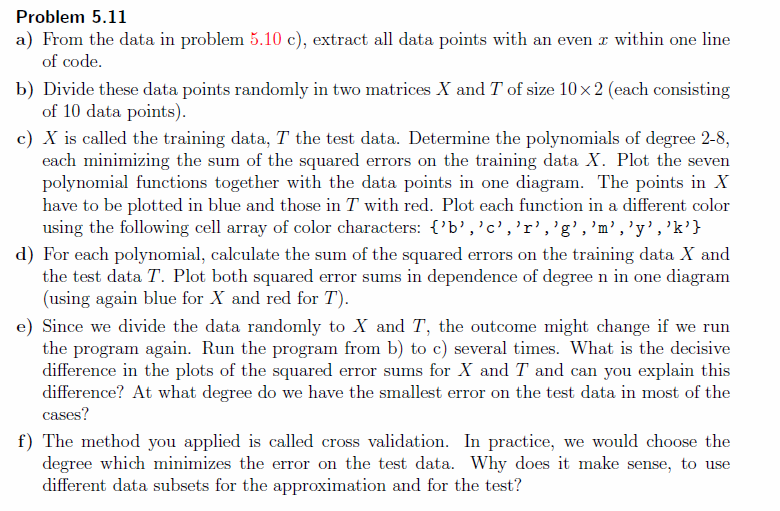
\includegraphics[width=1\textwidth]{chapters/images/desc-5-11}
\end{figure}


X

\begin{lstlisting}[caption=todo]

C

\end{lstlisting}

Y


\subsubsection{a)}

(getCoefficients und txtPoints von vorheriger Aufgabe) (ref zu Listing)

\begin{lstlisting}[caption=todo]


def myF8(x): return pow(x, 8);

def myF7(x): return pow(x, 7);

def myF6(x): return pow(x, 6);

def myF5(x): return pow(x, 5);

def myF4(x): return pow(x, 4);

def myF3(x): return pow(x, 3);

def myF2(x): return pow(x, 2);

def myF1(x): return x;

def myF0(x): return 1;


def getBaseFunctionList(degree):
	baseFunctions = [];
	
	if degree >= 8: baseFunctions.append(myF8);
	if degree >= 7: baseFunctions.append(myF7);
	if degree >= 6: baseFunctions.append(myF6);
	if degree >= 5: baseFunctions.append(myF5);
	if degree >= 4: baseFunctions.append(myF4);
	if degree >= 3: baseFunctions.append(myF3);
	if degree >= 2: baseFunctions.append(myF2);
	
	baseFunctions.append(myF1);
	baseFunctions.append(myF0);
	
	return baseFunctions;
#

def polynomialF(coefficients, x):
	sum = 0.0;
	
	nc = len(coefficients);
	
	for i in range(nc):
		sum += coefficients[i] * pow(x, nc - i - 1);
	
	return sum;
#


evenPoints = [];

for txtPoint in txtPoints:
	if txtPoint[0] % 2 == 0:
		evenPoints.append(txtPoint);


matrixX = [];
matrixT = [];

for evenPoint in evenPoints:
	rnd = random.random();
	
	if len(matrixT) >= 10 or (rnd < 0.5 and len(matrixX) < 10):
		matrixX.append(evenPoint);
	else:
		matrixT.append(evenPoint);



print("c)");

allYses = [];

xses = [];

for i in range(152):
	xses.append(8 + i * 0.25);


for i in range(7):
	degree = i + 2;
	
	baseFunctionList = getBaseFunctionList(degree);
	
	coefficients = getCoefficients(baseFunctionList, matrixX);
	
	yses = [];
	
	for x in xses:
		y = polynomialF(coefficients, x);
		yses.append(y);
	
	allYses.append(yses);


xXses = [];
xYses = [];
tXses = [];
tYses = [];

for i in range(10):
	xXses.append(matrixX[i][0]);
	xYses.append(matrixX[i][1]);
	tXses.append(matrixT[i][0]);
	tYses.append(matrixT[i][1]);


#colors = ["r", "g", "b", "c", "m", "y", "k"];
colors = ["b", "c", "r", "g", "m", "y", "k"];


plt.plot(xXses, xYses, "bo");
plt.plot(tXses, tYses, "ro");

for i in range(len(allYses)):
	plt.plot(xses, allYses[i], colors[i]);

plt.xlabel("x");
plt.ylabel("y");
plt.show();


print(" ");
print("d)");

def getError(coefficients, mat):
	errorSum = 0;
	
	for elem in mat:
		fY = polynomialF(coefficients, elem[0]);
		
		errorSum += pow(fY - elem[1], 2);
	
	return errorSum;
#

def getErrors(degree, matX, matT):
	baseFunctionList = getBaseFunctionList(degree);
	
	coefficients = getCoefficients(baseFunctionList, matX);
	
	errorSumX = getError(coefficients, matX);
	errorSumT = getError(coefficients, matT);
	
	return [errorSumX, errorSumT];
#

degrees = [];
errorsX = [];
errorsT = [];

for i in range(7):
	degree = i + 2;
	
	degrees.append(degree);
	
	errors = getErrors(degree, matrixX, matrixT);
	
	errorsX.append(errors[0]);
	errorsT.append(errors[1]);
#

plt.plot(degrees, errorsX, "b");
plt.plot(degrees, errorsT, "r");

plt.xlabel("degree");
plt.ylabel("error");
plt.show();


\end{lstlisting}


results:

\begin{lstlisting}[caption=Result of 1.1 a), keywordstyle=\color{black}]
R
\end{lstlisting}

X



\subsubsection{b)}

X

\begin{lstlisting}[caption=todo]

C

\end{lstlisting}


results:

\begin{lstlisting}[caption=Result of 1.1 a), keywordstyle=\color{black}]
R
\end{lstlisting}

X





\subsubsection{c)}

X

\begin{lstlisting}[caption=todo]

C

\end{lstlisting}


results:


\begin{figure}[!ht]
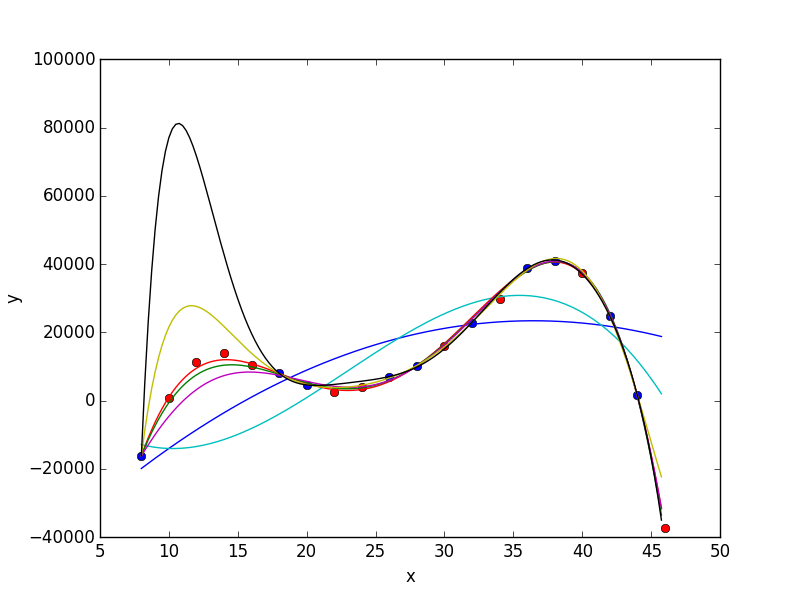
\includegraphics[width=1\textwidth]{chapters/images/figure-5-11-c}
\caption{todo}
\end{figure}

X



\subsubsection{d)}

X

\begin{lstlisting}[caption=todo]

C

\end{lstlisting}


results:


\begin{figure}[!ht]
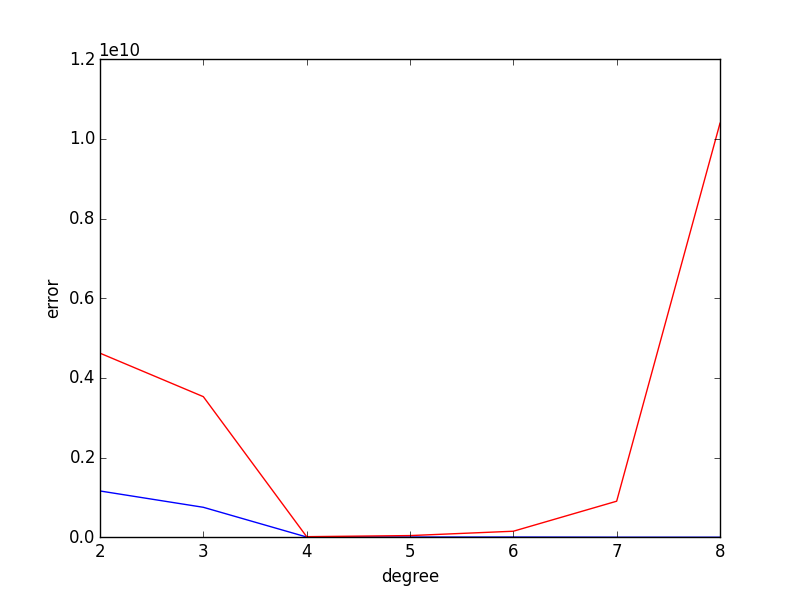
\includegraphics[width=1\textwidth]{chapters/images/figure-5-11-d}
\caption{todo}
\end{figure}

X





\subsubsection{e)}

The deviation to the original approximated function (where all data points were used) minimizes the more evenly the points of X and T are distributed. The reason for that is that when there's a large interval of test points only, the approximated function has no bounds at all in that interval and can deviate as much as it needs to, without increasing the error.
The results seems to be the the best with polynomials of degree 4 and 5.

\subsubsection{f)}


It makes sense because the approximated function is supposed to be close to all data values, and even the points "in between" which are not part of both the training and test data.